\section{Nine copper coins, and other toposes}\label{sec_coins}
\epigraph{
	Explicaron que una cosa es \emph{igualdad}, y otra \emph{identidad}, y formularon una especie de \emph{reductio ad absurdum}, o sea el caso hipotético de nueve hombres que en nueve sucesivas noches padecen un vivo dolor. ¿No sería ridículo -interrogaron- pretender que ese dolor es el mismo?\\[2mm]

	\footnotesize\emph{--- They explained that \emph{equality} is one thing and
	\emph{identity} another, and formulated a kind of \emph{reductio ad absurdum}: the
	hypothetical case of nine men who on nine nights suffer a severe pain. 
	Would it not be ridiculous -they questioned- to pretend that this pain is
	one and the same? }
}{JLB ---\tlon, Uqbar, Orbis Tertius}
The main result of the present section is a roundup of examples showing that it is possible to concoct categories of variable sets $\Set/I$ where some seemingly paradoxical constructions coming from J.L. Borges' literary world have, instead, a perfectly `classical' behaviour when looked in the internal logic of $\Set/I$.

Each of the examples in our roundup \autoref{bla}, \ref{bli}, \ref{blu} is organised as follows: we recall the statement in Borges' words. Then, we exhibit a topos in which the statement becomes admissible, when expressed in its internal language.
\subsection{Choosing an internal logic}
According to our description of the Mitchell-Bénabou language in the category of variable sets, \emph{propositions} are morphisms of the form
\[p : U \to \Omega_I\]
where $\Omega_I$ is the subobject classifier of $\Set/I$ described in \autoref{variable_sets_have_omega}; now, recall that
\begin{itemize}
	\item the object $\Omega_I = \Omega_0\times I \to I$ becomes an object of $\Set/I$ when endowed with the projection $\pi_I : \Omega_I \to I$ on the second factor of its domain ($\Omega_0$ is the subobject classifier of $\Set$, having a top element $\top$ and a bottom element $\bot$);
	\item the universal monic $\tr : I \to \Omega_I$ consists of a section of $\pi_I$, precisely the one that sends $i : I$ to the pair $(i,1) : \Omega_I$;
	\item every subobject $U \hookrightarrow A$ of an object $A$ results as a pullback (in $\Set/I$) along $\tr$:
	      \[\xymatrix@R=5mm@C=5mm{
		      U\ar[dr]^u\ar[rr]^u\ar[dd]_m&& I\ar[dd]^{\tr} \ar@{=}[dl]\\
		      &I& \\
		      A \ar[ur]\ar[rr]_{\chi_U}&& \ar[ul]\Omega_I
		      }\]
	      (see \autoref{variable_sets_have_omega} for a complete proof).
\end{itemize}
The set $I$ in this context acts as a \emph{multiplier} of truth values, in that every proposition can have a pair $(\epsilon, t)$ as truth value: $\epsilon$ is the truth value, `amplified' by $t : I$.
\begin{notation}
We introduce the following notation: a proposition $p : U \to \Omega_I$ is \emph{true} (resp. \emph{false}), in context $x :U$, with \emph{strength} $t$, if $p(x) =(1,t)$ (resp., $p(x)=(0,t)$). We say, in short, that $p$ is $t$-true in context $x:U$, and we denote these two judgments as
\[x:U\entails{t} p \qquad\qquad x:U\entails{t} \lnot p.\]
This notation is extensible in the obvious way:
\begin{itemize}
	\item $\vec x : U \entails{t} p$ means that $p(x_1,\dots,x_n) = (1,t)$ for $p : U= U_1\times\dots\times U_n\to \Omega_I$ and $\vec x = (x_1,\dots,x_n) : U$;
	\item $x : U \entails{t} p_1,\dots, p_n$ means that for every $1\le i \le n$ one has $p_i(x)=(1,t)$;
	      % \item $\vec x \entails{t} \vec p$, sometimes written at large
	      % \[
	      %   \bsmat x_1\\\vdots\\x_n \esmat \entails{t} \bsmat p_1\\\vdots \\ p_n \esmat
	      % \]
	      % means that in context $x_1 : U_1,\dots, x_n : U_n$ one has $p_j(x_j) = (1,t)$ for all $1\le j\le n$;
\end{itemize}
every other combination is similarly defined.
\end{notation}
This notation is chosen in order not to make explicit reference to the set of truth values we take for our background logic in $\Set$; all the results that we state independent from the assumption that the subobject classifier $\Omega_0$ of $\Set$ is the usual two-element Boolean algebra $\{0 < 1\}$. (This will be, however, our natural choice.)

Some of the usual introduction and elimination rules apply to the $\entails{t}$ judgment, for example
\[\infer[\Pi\textsc{-intro}]{(a,b) : A\times B \entails{t} p}{a : A \entails{t} p(\firstblank,b) & & b \entails{t} p(a,\firstblank)}\]
This is not accidental; however, we will not say more on the structure of the deductive system so generated, as it would derange us from our main topic of discussion.
\begin{remark}\label{very_importanta_force}
	A proposition in the internal language of variable sets is a morphism of the following kind: a function $p : U \to \Omega_I$, defined on a certain domain, and such that
	\[
		\xymatrix{
			U\ar[d]_u\ar[r]^-p  & \Omega_0\times I \ar[d]^{\pi_I}\\
			I \ar@{=}[r]& I
		}
	\]
	(it must be a morphism of variable sets!) This means that $\pi p(x : U) = u(x : U)$, so that $p(x) = (\epsilon_x, u(x))$ for $\epsilon_x =0,1$ and $u$ is uniquely determined by the `variable domain' $U$. We can succintly denote this fact in the above notation, writing
	\begin{equation}\label{entailment} \infer{x : (U,u) \entails{u(x)} \epsilon_x\cdot p}{}\end{equation}
	where $\epsilon_x \cdot p$ is $p$ if $\epsilon_x=1$, and $\lnot p$ otherwise.

	This is an important observation: the strength with which $p$ is true/false is completely determined by the structure of its domain, in the form of the function $u : U \to I$ that renders the pair $(U,u)$ an object of $\Set/I$.
\end{remark}
\begin{remark}\label{something_on_I}
	To get a concrete grip on the different classes of propositions we  can build in an internal language, it is now convenient to restrain the structure of $I$ in order to satisfy our intuition that it is a space of \emph{strengths}: it is for example possible to equip $I$ with an order structure, or a natural topology.

	Among all such different choices of truth multiplier, yielding different categories of variable sets, and different kinds of internal logic therein, we will concentrate our study on $I$'s that are dense, linear orders with LUP; thus not really far from being a closed, bounded subset of the real line.\footnote{There is another more philosophical reason for this assumption, that will appear clear throughout the section: density of $I$ is meant to allow `intersubjective concordance' between two interlocutors $X$ and $Y$. Engaging in a debate on existence of the nine coins, $X,Y$ might disagree about how strongly some of them exist; the assumption that $I$ is a dense order makes it possible to always find an intermediate strength between the one $p_X$, assigned by $X$, and the one $p_Y > p_X$ assigned by $Y$ to the same set of coins, as there must be a third truth value $z:p_X < z < p_Y$ lying between the two.}
\end{remark}
Even if this assumption is never strictly necessary, a natural choice for $I$ is a \emph{continuum} (=a dense total order with LUP --see \cite{moschovakis2009descriptive}), a basic model of which is the closed unit interval $[0,1]$ of the real line.

An alternative choice drops the density assumption: in that case the (unique) finite total order $\Delta[n] = \{0 < 1 <\dots < n\}$, or the countable total order $I=\omega = \{0,1,2,\dots,n,\dots\}$ are all pretty natural choices for $I$ (although it is way more natural for $I$ to have a minimum \emph{and} a maximum element).\footnote{We're only interested in the notion of an abstract interval here: a continuum $X$ endowed with an operation $X \to X \vee X$ of `zooming', uniquely defined by this property. In a famous paper Freyd characterises `the interval' as the terminal interval coalgebra: see \cite[§1]{freyd2008algebraic}; for our purposes, note that $[0,1]$ is a natural choice: it is a frame, thus a Heyting algebra $\fkH =([0,1],\land,\lor,\Rightarrow)$ with respect to the pseudo-complement operation given by $(x \Rightarrow z) := \bigvee_{x\land y \le z} y$ (it is immediate that $x \land a \le b$ if and only if $a \le x \Rightarrow b$ for every $a,b: [0,1]$).}
\begin{remark}\label{fig_Omega}
	In each of these cases `classical' logic is recovered as a projection: propositions $p$ can be true or false with strength $1$,\footnote{Here $I$ is represented as an interval whose minimal and maximal element are respectively $0$ and $1$; of course these are just placeholders, but it is harmless for the reader to visualise $I$ as the interval $[0,1]$.} the maximum element of $I$:
	\begin{center}
		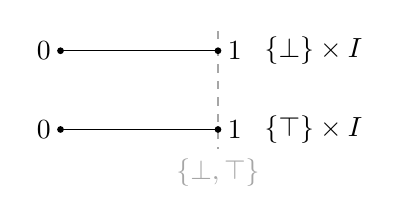
\begin{tikzpicture}
			\draw[gray!70,dashed] (2,1.25) -- (2,-.25) node[below] {$\{\perp,\top\}$};
			\draw[fill] (0,0) circle (1pt) node[left] {$0$};
			\draw[fill] (2,0) circle (1pt) node[right] (dis) {$1$};
			\draw (0,0) -- (2,0);
			\begin{scope}[yshift=1cm]
				\draw[fill] (0,0) circle (1pt) node[left] {$0$};
				\draw[fill] (2,0) circle (1pt) node[right] (dat) {$1$};
				\draw (0,0) -- (2,0);
				\node[right of=dis] {$\{\top\}\times I$};
				\node[right of=dat] {$\{\perp\}\times I$};
			\end{scope}
		\end{tikzpicture}
	\end{center}
\end{remark}
In order to aid the reader understand the explicit way in which $I$ `multiplies' truth values, we spell out explicitly the structure of the subobject classifier in $\Set/\Delta[2]$. In order to keep calling the minimum and maximum of $I$ respectively $0$ and $1$ we call $\frac{1}{2}$ the intermediate point of $\Delta[2]$.
\begin{remark}
	The subobject classifier of $\Set/\Delta[2]$ consists of the partially ordered set $\Delta[1]\times\Delta[2]$ that we can represent pictorially as a rectangle
	\[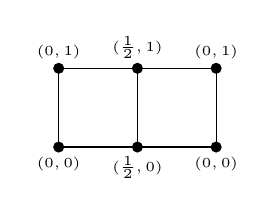
\begin{tikzpicture}[xscale=2]
			\foreach \i/\name in {0/0,.5/{\frac{1}{2}},1/0}{
			\foreach \j/\pos in {0/below,1/above}
			\fill (\i,\j) ellipse (1pt and 2pt) node[\pos] {\tiny $(\name,\j)$};
			}
			\draw (0,0) rectangle (1,1);
			\draw (.5,1) -- (.5,0);
		\end{tikzpicture}\]
	endowed with the product order. The resulting poset is partially ordered, and in fact a Heyting algebra, because it results as the product of two Heyting algebras: the Boole algebra $\{0<1\}$ and the frame of open subsets of the Sierpiński space $\acute{S} =(\{a,b\}, \tau_S)$ (the topology is $\tau_S = \{\varnothing, \{a\}, \{a,b\}\}$).
\end{remark}
\begin{remark}\label{alcuni_set}
	Given that $I=[0,1]$ endowed with its usual Euclidean topology is one of our most natural choices, we explicitly define some interesting sets obtained out of $\Omega_I$ or out of a given proposition $p : U \to \Omega_I$ in the Mitchell-Bénabou language of $\Set/[0,1]$:
	\begin{itemize}
		\item the two sets
		      \begin{align*}
			      A^\top  & = \big\{x:U\entails{t_x} p,\, t_x > 0\big\}\subseteq U        \\
			      A^\perp & = \big\{x:U \entails{t_x} \lnot p,\, t_x > 0\big\}\subseteq U
		      \end{align*}
		      the last set is canonically identifies to the subset of structure functions $\cvar{U}{u}{I}$ such that $u^\leftarrow 0 = \varnothing$.
		      % \item Similarly, we define $Z^\top = p^\leftarrow(\{\top\}\times [0,1))$ and its companion $Z^\bot$.
		\item the two sets
		      \begin{align*}
			      B^\top  & = \big\{ x:U \entails{1} p \big\}\subseteq U       \\
			      B^\perp & = \big\{ x:U \entails{1} \lnot p \big\}\subseteq U
		      \end{align*}
		      these are obtained as fibers over the maximal element of $I$. A useful shorthand for the judgment $\entails{1}$ is just $\entails{}$.
		\item the two sets
		      \begin{align*}
			      E_t^\top  & = \{ x : U \entails{t} p\}\subseteq U       \\
			      E_t^\perp & = \{ x : U \entails{t} \lnot p\}\subseteq U
		      \end{align*}
		      Clearly, $B^\top = \coprod_{t : I} E_t^\top$ and $B^\bot = \coprod_{t : I} E_t^\bot$.
	\end{itemize}
\end{remark}
A crucial decision at some point will be about the regularity with which the strength of $p$ depends with respect to the variables on its domain of definition. Without a continuous dependence, small changes in context $x : U$ might drastically change the truth value $p(x)$.\footnote{There is no a priori reason to maintain that $p$ is a continuous proposition; one might argue that discontinuous changes in truth value of $p$ happen all the time in `real life'; see the family of paradoxes based on so-called \emph{separating instants}: how well-defined the notion of `time of death' is? How well-defined the notion of `instant in time'?}
\subsection{The unimaginable topos theory hidden in Borges' library}
Jorge Luis Borges' literary work is well-known to host paradoxical worlds; oftentimes, seemingly absurd consequences follow by stretching ideas from logic and Mathematics to their limits: time, infinity, self-referentiality, duplication, recursion, the relativity of time, the illusory nature of our perceptions, eternity as a curse, the limits of language, and its capacity to generate worlds.

In the present section, we choose \emph{Fictions}, Borges' famous collection of novels, as a source of inspiration to put to the test possible and impossible worlds together with their ontology.

In a few words, Borges' work generates `impossible worlds': the term as it is is used in various ways in paraconsistent semantics since the classic work of Rescher and Brandom \cite{10.2307/20127724}, where worlds are obtained starting from `possible' ones, through recursive operations on standard Kripkean worlds.

Here we claim that interesting consequences originate from reversing the above perspective: instead of removing from the realm of possibility those worlds that do not comply with sensory experience tagging them as `impossible', we accept their existence, for bizarre that it may seem, and we try to deduce ex post, \emph{from their very existence}, a kind of logic that can consistently generate them.

The results of our analysis are surprising:
\begin{itemize}
	\item we unravel how a mathematically deep universe Borges has inadvertently created: of the many compromises we had to take in order to reconcile literature and the underlying Mathematics,\footnote{See \autoref{our_beloved_interval} below: these compromises mainly amount to assumptions on the behaviour of space-time on \tlon and Babylon.} we believe no one is particularly far-fetched;
	\item we unravel how ontological assumptions are context-dependent; they are not given: using category theory ontology, far from being the presupposition on which language is based, is a byproduct of language itself. The more expressive language is, the more expressive ontology becomes; the fuzzier its capacity to assert truth, the fuzzier ontology becomes;
	\item since `fuzziness' of existence, i.e. the fact \emph{entia} exist less than completely, is hard-coded in the language (in the sense of \autoref{da_lang}) of the category we decide to work in from time to time, most of the statements of \tlon's ontology are paradoxical only when regarded with Earthlings' eyes; on \tlon they are, instead, perfectly legitimate statements.
\end{itemize}
To sum up, readers willing to find an original result in this paper might find it precisely here: we underline how Borges' alternative worlds (Babylon, \tlon \ dots) are mathematically consistent places, worthy of existence as much as our world, only based on a different internal logic.

\subsubsection{Nine copper coins} The first paradox we aim to frame in the right topos is the famous nine copper coins argument, used by the philosophers of Tlön to construct an impossible object persisting to exist over time, even without a perceivent that maintains it in a state of being.
\begin{example}[Nine copper coins]\label{bla}
	First, we recall the exact statement of the paradox:\footnote{The paradox appears in a primitive, mostly unchanged version in \cite{borges1997otras}, where instead of nine copper coins, a single arrow, shot by an anonymous archer, disappears among the woods. For what concerns \tlon's  nine copper coins, our translation comes from \cite{tlonEN}:
		\begin{quote}
			Tuesday, $X$ crosses a deserted road and loses nine copper coins. On Thursday, $Y$ finds in the road four coins, somewhat rusted by Wednesday's rain. On Friday, $Z$ discovers three coins on the road. On Friday morning, $X$ finds two coins in the corridor of his house. The heresiarch would deduce from this story the reality - i.e., the continuity - of the nine coins which were recovered.

			It is absurd (he affirmed) to imagine that four of the coins have not existed between Tuesday and Thursday, three between Tuesday and Friday afternoon, two between Tuesday and Friday morning. It is logical to think that they have existed - at least in some secret way, hidden from the comprehension of men - at every moment of those three periods.
		\end{quote}}
	\begin{quote}
		El martes, $X$ atraviesa un camino desierto y pierde nueve monedas de cobre.
		El jueves, $Y$ encuentra en el camino cuatro monedas, algo herrumbradas por la lluvia del miércoles. El viernes, $Z$ descubre tres monedas en el camino. El viernes de mañana, $X$ encuentra dos monedas en el corredor de su casa. El  quería deducir de esa historia la realidad -id est la continuidad- de las nueve monedas recuperadas.

		Es absurdo (afirmaba) imaginar que cuatro de las monedas no han existido entre el martes y el jueves, tres entre el martes y la tarde del viernes, dos entre el martes y la madrugada del viernes. Es lógico pensar que han existido -siquiera de algún modo secreto, de comprensión vedada a los hombres- en todos los momentos de esos tres plazos.
	\end{quote}
	Before going on with our analysis, it is important to remark that there is one and only one reason why the paradox of the nine copper coins is invalid: copper does not rust. Incidentally, we will be able to propose a rectification of this `rust counterargument' without appealing to the cheap assumption that copper can rust on \tlon due to a purported difference between Earth's and \tlonian chemistry.

	Expressed in natural language, our solution to the paradox goes more or less as follows: $X$ loses their coins on Tuesday, and the strength $\varphi$ with which they `exist' lowers; it grows back in the following days, going back to a maximum value when $X$ retrieves two of their coins on the front door. $Y$ finding of other coins raises their existence strength to a maximum. The coins that $Y$ has found rusted (more precisely, with their surface slightly oxidized: this is possible, but water is rarely sufficient to ignite the process alone --certainly not in the space of a few hours).
	\begin{remark}\label{our_beloved_interval}
		In this perspective, \tlon classifier of truth values can be taken as $\Omega_I = \{0<1\}\times I$, where $I$ is any set with more than one element; a minimal example can be $I=\{N,S\}$,\footnote{Justifying this choice from inside \tlon is easy: the planet is subdivided into two hemispheres; each of which now has its own logic `line' independent from the other.} but as explained in \autoref{our_beloved_interval} a more natural choice for our purposes is the closed real interval $I=[0,1]$.

		This allows for a continuum of possible forces with which a truth value can be true or false;  it is to be noted that $[0,1]$ is also the most natural place on which to interpret fuzzy logic, albeit the interest for $[0,1]$ therein can be easily and better motivated starting from probability theory.\footnote{Tangential to our discussion might be the fact that there are interesting perspective on how to develop basic measure theory out of $[0,1]$. For example, measures valued in things like Banach space and more general topological  vector spaces have been considered.}
	\end{remark}
	We now start to formalise properly what we said until now. To set our basic assumptions straight, we proceed as follows:
	\begin{itemize}
		\item Without loss of generality, we can assume the set $C = \{c_1,\dots,c_9\}$ of the nine coins to be totally ordered and partitioned in such a way that the first two coins are those retrieved by $X$ on Tuesday, the subsequent four are those found by $Y$ on their way, and the other three are those seen by $Z$ on Friday. So,
		      \[C = C_X \sqcup C_Y \sqcup C_Z\]
		      and $C_X = \{c_{X1}, c_{X2}\}$, $C_Y = \{c_{Y1},c_{Y2},c_{Y3},c_{Y4}\}$, $C_Z= \{c_{Z1}, c_{Z2}, c_{Z3}\}$ As already said, the truth multiplier $I$ is the closed interval $[0,1]$ with its canonical order --so with its canonical structure of Heyting algebra, and if needed, endowed with the usual topology inherited by the real line.
		\item Propositions of interest for us are of the following form:
		      \[\lambda gcd.p(g, c, d) : \{X,Y,Z\}\times C\times W \to \Omega_I\]
		      where $W \subseteq \{\S,\M,\Tu,\W, \Th,\F,\Sa\}$ is a set of days (strictly speaking, the paradox involves just the interval between \Tu (Tuesday) and \F (Friday). The value $p(g,c,d)$ models how in $g$'s frame of existence the coin $c$ exists at day $d$ with strength $p(g,c,d)$.
	\end{itemize}
	\begin{definition}[Admissible configuration]
		We now define an \emph{admissible} configuration of coins any arrangement of $C$ such that the following two conditions are satisfied:
		\begin{enumtag}{ad}
			\item \label{ad:uno} for all day $d$ and coin $c$, we have
			\[
				(g,c,d) : G\times C\times W \entails{} p
				%\sum_{u: \{X,Y,Z\}} p(u,c,d) = (\top, 1)
			\]
			where we denote as `sum' the logical conjunction in $\Omega_I$: this means that day by day, the \emph{global} existence of the group of coins constantly attains the maximum; it is the \emph{local} existence that lowers when the initial conglomerate of coins is partitioned.
			\item \label{ad:due} Moreover, all these conditions holds:
			\begin{align*}
				% \sum_{c_X: C_X} p(X,c_X,\F) = (\top,1) \\
				% \sum_{c_Y: C_Y} p(Y,c_Y,\Th) = (\top,1) \\
				% \sum_{c_Z: C_Z} p(Z,c_Z,\F) = (\top,1)
				(X,\F)  & \entails{} \textstyle \sum_{c_X} p(\firstblank,c_X,\secondblank)  \\
				(Y,\Th) & \entails{} \textstyle \sum_{c_Y} p(\firstblank,c_Y,\secondblank)  \\
				(Z,\F)  & \entails{} \textstyle \sum_{c_Z} p(\firstblank,c_Z,\secondblank),
			\end{align*}
			meaning that, for example in the first case, $\sum_{c_X} p(X,c_X,\F) = (\top,1)$.
		\end{enumtag}
	\end{definition}
	In an admissible configuration the subsets $ C_X, C_Y, C_Z $ can only attain an existence $p(g,c,d) \lneq (\top,1)$; that is to say, \emph{no coin completely exists locally}. But for an hypothetical external observer, capable of observing the system, adding up the forces with which the various parts of $C$ exist, the coins \emph{globally} exist ` in some secret way, of understanding forbidden to men' (or rather, to $ X, Y, Z $).
	\begin{center}
		\begin{figure}[h]
			\begin{tikzpicture}[xscale=6, yscale=4]
				\coordinate (1) at (0,0);
				\foreach \i/\j in {1/\W,2/\Th,3/\F}{
						\draw[gray!90] (\i/4,0) node[below] {\tiny \j} -- (\i/4,1);
					}
				\node[below,gray!90] at (0,0) {\Tu};
				\node[below,gray!90] at (1,0) {\Sa};
				\coordinate (1) at (0,0);
				\coordinate (2) at (1/2, 1/5);
				\coordinate (3) at (3/4,1);
				\draw[thick,red]
				(1) .. controls ++(.25,.25) and (.25,.5) .. (2)
				node[right] {\scriptsize $1/5$}
				.. controls (.625,0) and (.75,.25) .. (3);
				\draw[thick,green!40!black] (1) -- (2) -- (3);
				\draw[thick,blue] (1)
				.. controls (.275,.25) and (0,1) .. (1/2,1) node[above] {\scriptsize $p(Y, c_Y)=(\top,1)$}
				%   .. controls (1,1) and (.5,.25) .. 
				-- (3/4,1/4) node[right] {\scriptsize $1/4$};
				\node[fill=gray!60] (cloud) at (1/4,1/2) {\large\color{black} \faCloud};
				\draw[thick] (0,1) |- (1,0);
			\end{tikzpicture}
			\caption{A pictorial representation of the truth forces of coins in different days; we choose a minimally complex model where strength of existence goes up and down to join the points where \cite{tlonEN} gives complete information about the coins' configuration. $X$ is marked in red, $Z$ in yellow, $Y$ in blue. Time is considered as a continuum line, marked at weekdays for readability.}
			\label{fig_coins}
		\end{figure}
	\end{center}
\end{example}
\begin{remark}
	Lest the reader think our construction is just a sleight of hand leaving open the main problem posed by the coin riddle, an important clarification is now in order: \emph{where} do the coins exist? This is a problematic question. \tlon's idealist might deny time (our model makes no strong assumption on what time is made of: discrete, continuous, homogeneous, slowed by traveling at high speed\dots); $B^\top$ ontologists live comfortably in $B^\top$, as defined in \autoref{alcuni_set} without being able to tell anything about how objects `completely do not exist'.

	At the opposite side of the spectrum the pure empiricist lives in $B^\bot$, and they're unable to tell how they `completely exist').

	This is where our analysis comes in handy; in particular, this is where our particular choice of $\Omega_I$ plays its r\^ole. In our model $B^\perp, B^\top$ both result as disjoint sum of slices, each of which collects the particular fibers $E_t^\perp, E_t^\top$ of \ref{alcuni_set}; looking at $ \coprod_{t : I} E_t^\top$ and $ \coprod_{t : I} E_t^\bot$ is a genuinely better approach than just considering $B^\perp, B^\top$ as atomic, since it yields a precise quantification of \emph{how much} something does (not) exist, framing both $B^\top$- and $B^\bot$-ontologies as opposite sides of a spectrum made out of diverse colours.
\end{remark}
\begin{example}
	An example of an admissible configuration of coins is the following (cf. \autoref{fig_coins}): we assume strength of existence varies joining the points where \cite{Borges1963} gives us complete information about the existence status of $C_X,C_Y,C_Z$ above: in the remaining instants of time, the coins out of sight for $X$ share an equal amount of existence in such a way that constraints \ref{ad:uno} and \ref{ad:due} above are satisfied: in this particular example, $p(Y,c_Y,\Th) = (\top,1)$, whereas $p(X,C_X,\Th)=p(Z,C_Z,\Th)=(\top,1/5)$, and $p(Y,c_Y,\F)=(\top,1/4)$, whereas $p(X,C_X,\F)=p(Z,C_Z,\F)=(\top,1)$.

	Certainly the reader will have fun finding different possible admissible configurations of coins, and building themselves additional details to enrich the bare story of $X,Y,Z$ (for example: can the cardinality of $\{X,Y,Z\}$ depend on $I$? If yes, how?).
\end{example}
\subsubsection{Continuity and discontinuity} Continuity and discontinuity of a proposition $p : U \to \Omega_{[0,1]}$ now capture quite well other pieces of Borges' literary universe: here we provide two examples. We refrain from a deep, quantitative analysis, and we invite the reader to fill the details of our reasoning as a pleasant re-reading exercise of \cite{babil} and \cite{tlonEN}.\footnote{The plot of \cite{babil} in a nutshell is: in Babylon, a lottery game infiltrates reality to the point that it ends up governing the actions of all men; liberating them from free will while coorting them into pawns of an infinite, inescapable, unknowable game, governed by an iron, seemingly chaotic, probabilistic logic.}
\begin{remark}[Continuity for a proposition]\label{continuiti}
	Let $p : U \to \Omega_I$ be a proposition; here we investigate what does it mean for $p$ to be (globally) continuous with respect to the Euclidean topology on $I=[0,1]$, in the assumption that its domain of definition $U$ is metrisable (this is true for example when $U$ is a subset of space-time). The condition is that
	\[ \forall \epsilon > 0,\,\exists \delta > 0 : |x-y|< \delta \To |px-py| < \epsilon. \]
	In layman terms: $p$ is continuous on its domain of definition if its strength over nearby events can't change too dramatically.

	All elementary topology results apply to such a proposition: for example, the set of forces with which $p$ is true or false is a connected subset of $\Omega_{[0,1]}$, compact if $U$ was compact.
\end{remark}
\begin{example}[Discontinuity, sapphire from Taprobana]\label{bli}
	Propositions $p : U \to \Omega_{[0,1]}$ that are allowed to be discontinuous in its variables depend unpredictably from their context: such propositions model seemingly chaotic events triggered as the end terms of a chain of disconnected prior events; in fact, if we assume a real base for the domain of $p$, its continuity as stated in \autoref{continuiti} roughly means that events in the same neighbourhood --`near' in space or temporally contiguous-- can't have too much different truth/strength values.

	A model for such a universe, where `terrible consequences' sometimes follow from the `impersonal drawings, whose purpose is unclear' characterising the Company's actions: seemingly disconnected (that `a sapphire from Taprobana be thrown into the waters of the Euphrates'; that `a bird be released from the top of a certain tower'; that `every hundred years a grain of sand be added to (or taken from) the countless grains of sand on a certain beach'), but generating nontrivial dynamics when inserted in a suitable sequence as in \autoref{fig_dynamics}.

	Let us consider the dynamical system $([0,1],\nabla\circ p)$ (see \autoref{dyn_sisy}) obtained from the iterates of the composition $\nabla \circ p : [0,1] \to [0,1]$ ($\nabla : I\amalg I \to I$ is the fold map of $I$, obtained from the identity of $I$ and the universal property of the coproduct). We start from a proposition $p$ depending on a free variable $t : I$; then, $p(t) = (u(t),\epsilon): \Omega_I$ consists of a strength and a truth value; but $p$ can be evaluated on $u(t)$ because of \eqref{entailment} ($u$ is a continuous endomorphism of a compact metric space; although this is not its universal property, the fold map $\nabla$ just forgets the truth value, keeping the force):
	\[
		t : I\entails{u(t)} p \qquad u(t) :I \entails{u(u(t))} p \qquad \dots
	\]
	The process can thus be iterated as follows, exploiting the universal property of the natural number object in $\Set/I$:
	\begin{center}
		\begin{figure}[h]
			\def\line{\draw (0,0) -- (1,0); \draw (0,.5) -- (1,.5);}
			\begin{tikzpicture}
				\line
				\fill (.395,0) circle (1pt);
				\foreach \i/\j/\k in {2.25/.382/0,4.5/.537/.5,6.75/.874/.5,9/.128/0}{
						\begin{scope}[xshift=\i cm]
							\line
							\fill (\j,\k) circle (1pt);
							\node at (-.5,.375) {$\overset{\scriptscriptstyle\nabla\circ p}\mapsto$};
						\end{scope}
					}
			\end{tikzpicture}
			\caption{A dynamical system induced by the Company's infinite, impersonal drawings.}
			\label{fig_dynamics}
		\end{figure}
	\end{center}
	It is clear that the limit behaviour of such a sequence strongly depends on the analytic properties of $u$ (e.g., if $u$ is a contraction, it must have a single fixed point). A repeated series of drawings can chaotically deform the configuration space on which $p$ is evaluated. There is of course countless termination conditions on such process $p$; the series can be periodic, it can stop when $p$ reaches maximum or minimum force, or a prescribed value, when $u$ reaches its unique fixed point --if any, or is inside/outside a certain range of forces\dots; we leave such speculations to the mystagogues of the Company, or to the lions of Qaphqa.
\end{example}
Another compelling example is that of the monotonicity of a proposition depending, say, on a certain number of observers who acknowledge the `existence' of an object $R$ (be it physical or conceptual) in large numbers, from which very reason the existence of $R$ gains strength.
\begin{example}[Continuity: a few birds, a horse]\label{blu}
	Let us consider objects whose existence strength depends \emph{monotonously} and continuously from their parameters: for example a proposition $p$ may be `truer' the more people observe it, because
	\begin{quote}
		things became duplicated in Tlön; they also tend to become effaced and lose their details when they are forgotten. A classic example is the doorway which survived so long it was visited by a beggar and disappeared at his death. At times some birds, a horse, have saved the ruins of an amphitheater.  \hfill\cite{tlonEN}
	\end{quote}
	In such a situation, we can note that the strength of existence of some ruins --modeled as it is the more naive to do, like a rigid body $R$ in space-- depends on the number of its observers:
	\[(R,n)\entails{1-\frac{1}{n}} p.\]%\textstyle p(R, n) = \big(\top, 1-\frac{1}{n}\big)\]
	\begin{figure}[h]
		\begin{center}
			\begin{tikzpicture}[xscale=1.25]
				\draw[->, thick, >=stealth] (0,0) -- (6,0);
				\foreach \j/\i in { 1/.2
						, 2/.35
						, 3/.55
						, 4/.8
						, 5/1
					}
				\node[opacity=\i] at (\j,.65) {\fontsize{30}{30}\selectfont \Tribar};
			\end{tikzpicture}
		\end{center}
		\caption{On \tlon, there are things that exist stronger the more you believe in them. This is a consequence of the strength $p(\Tribar)$ monotonically depending on an increasing variable $n$ (`trust' in that existence, `belief' that the impossible tribar \Tribar exists.)}
	\end{figure}
\end{example}
\subsubsection{Changing the geometry of $I$}
To conclude the section, a last --somewhat dramatic-- example. What happens if we change topology on $I$? For example, we could brutally forget the Euclidean topology of the closed interval $[0,1]$, and regard $I$ as the disjoint union $\{ \{t\} \mid t: [0,1]\}$ of its points; so, the subobject classifier becomes the disjoint union of $[0,1]$ copies of $\{\perp,\top\}$. (See \autoref{fig:berkeley} below for a picture.)
\begin{example}[Burning fields at the horizon]\label{incendiata}
	The main tenet of the present paragraph is that Berkeley idealism of infinite and disconnected instants of time finds a natural home in our framework if the classifier is chosen to be the object $\Omega_I = \coprod_{t : [0,1]} \{ \perp,\top\}$. Such a peculiar logical framework allows for language to be reshaped in light of Berkeleyan instantaneism: the various terms of the perceptual bundle are recorded and stockpiled by instantaneous accretion, by disjoint sum of their constituents. This is exactly what happens on \tlon for words like `round airy-light on dark' or `pale-orange-of-the-sky'; objects are determined by their simultaneity, instead of their logical dependence: accretion superimposes fictitious meaning on a temporal sequence; it is just an illusion, a mistake of perception tricked into an illicit interpolation.
	\begin{quote}
		\hspace{.5em} Spinoza ascribes to his inexhaustible divinity the attributes of extension and thought; no one in Tlön would understand the juxtaposition of the first (which is typical only of certain states) and the second - which is a perfect synonym of the cosmos. In other words, they do not conceive that the spatial persists in time. The perception of a cloud of smoke on the horizon and then of the burning field and then of the half-extinguished cigarette that produced the blaze is considered an example of association of ideas.   \hfill\cite{tlonEN}
	\end{quote}
	\begin{center}
		\begin{figure}[h]
			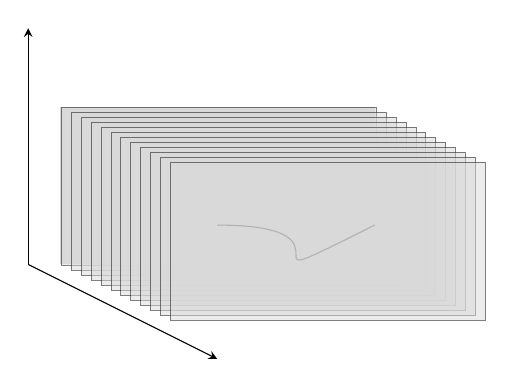
\begin{tikzpicture}[xscale=4, yscale=2]
				\fill[gray!30] (0,0) rectangle (1,1);
				\foreach \i in {.1,1,...,10}
				\draw[xshift=\i, yshift=-\i, ultra thin, fill=gray!30, opacity=.5] (0,0) rectangle (1,1);
				\draw[->, >=stealth, thin] (-.1,0) -- (-.1,1.5);
				\draw[->, >=stealth, thin] (-.1,0) -- (.5,-3/5);
				\draw[gray!60, xshift=.5cm, yshift=.25cm] (0,0) .. controls (.5,0) and (0,-.5) .. (.5,0);
			\end{tikzpicture}
			\caption{Time as an infinite, and infinitely subdivided, sequence of distinguished instants: the `Berkeley paradox' of non existence of causality lives in a certain topos, as nearby slices $E_t, E_s$ for small $|s-t|$ give no predictive power on how (and if) the transition from $E_t$ to $E_s$ might happen.}
			\label{fig:berkeley}
		\end{figure}
	\end{center}
\end{example}
Instantaneism is, of course, way larger a topic to cover than a paragraph could do. However, we attempt to scratch the surface of this fascinating topic in our \autoref{berkelei} below, where we sketch a possible `rebuttal to the idealist': it is entirely possible the world is affected in some way by me closing my eyes: thus, Berkeley has a fragment of a point. Yet, it takes more than that to make it disappear; thus, Berkeley is obviously wrong.

As always, Truth lies in the middle (of a continuous interval): observation --or lack thereof-- affects beings (more: it affects \emph{Being}) so that something changes in the assertion $p$ that `Everything exists' with my eyes open, and with my eyes closed.

This difference shall be regarded as an infinitesimal dent on $p$'s strength of truth, so to let Berkeleyan idealism gain a little ground. Yet, it is improper to say that the world `vanished'. It didn't for the rest of you.

The best we can say is that $p$ probably depends --monotonically-- on the number of open eyes. After all, objects on \tlon double, triple, they are cyclically reborn; they vanish as the doorway which survived `so long it was visited by a beggar and disappeared at his death'.